% !TeX root = ejemplo-memoria.tex
\documentclass[twoside,spanish,a4paper,12pt]{tfg}

% Editar la titulación
\titulacion{Grado en Ingeniería \\ Informática}

% Editar el título
\title{Trabajos con Interfaz Cerebro-Computador}

% Si es una alumna se debe usar
% \authorlabel{Autora}
\authorlabel{Autora}
% Editar el nombre
\author{Lucía Montañana Fuentes}


% Si hay varios tutores:
% \tutorlabel{Tutores}
% \tutor{Nombre del tutor 1 \\[2mm] Nombre del turor2}
% Si el tutor es masculino:
% \tutorlabel{Tutor}
\tutorlabel{Tutor}
% Editar
\tutor{Jose Vicente Riera López}

% Editar: Poner mes y año de la convocatoria de lectura del TFM
\convocatoria{Julio 2025}

\begin{document}

% NO QUITAR ESTOS ELEMENTOS
\portada
\cleardoublepage
\contraportada
\cleardoublepage
\declaracion
\cleardoublepage


% Editar: Resumen en Español (obligatorio)
\begin{resumen}
  A día de hoy el campo de la interacción con objetos a través de impulsos cerebrales esta en la alza, este trabajo se centra en analizar el estado actual y las aplicaciones de esta plataforma de hardware abierto en neurociencia, biomedicina e interfaces cerebro-computadora. El hardware de OpenBCI destaca por su accesibilidad y versatilidad, siendo una alternativa open source frente a soluciones comerciales en la adquisición y análisis de señales biomédicas como EEG, EMG y ECG. Actualmente, estas tecnologías están en constante expansión, facilitando investigaciones sobre control por pensamiento, rehabilitación cognitiva y análisis emocional. En esta tesis tenemos un hardware no invasivo para poder investigar las posibles utilidades. En concreto vamos a usar el casco con la placa Cyton complementandola con la placa Daisy para registrar ondas EEG.
\end{resumen}
\cleardoublepage

% Editar: Resumen en Inglés
\begin{abstract}
  This is the abstract of the TFM. It must be short and cover the main aspects of the TFM.
\end{abstract}
\cleardoublepage

\cleardoublepage


% Editar: Agradecimientos (opcional)
\begin{agradecimientos}
  En primer lugar a mis padres por aguantar los años de carrera que me queria matar y dejarlo constantemente.

  En segundo lugar a mis amigos que he hecho durante esta puta tortura, sin vosotros no podría haber superado este infierno de carrera, me habéis enseñado a trabajar en equipo siempre, a colaborar y a salir siempre de los peores agujeros. 

  En tercer lugar los amigos de fuera de esta cueva parasitaria, por estar siempre ahí, por haber entrado conmigo y haber salido conmigo también, sois la familia que elegí y estoy tan agradecida de haberos elegido. 
\end{agradecimientos}
\cleardoublepage

\tableofcontents

\pagestyle{tfg}
\justify

% Las figuras se buscan en el directorio figs

% Cada capítulo está en su propio fichero tex. Ver el directorio tex.

% La bibliografía está dentro del directorio bib
\chapter{Introducción}
% Contenidos del capítulo.
% Las secciones presentadas son orientativas y no representan
% necesariamente la organización que debe tener este capítulo.

\section{Introducción}
Las tecnologías OpenBCI son una herramienta fundamental de la investigación de neurocientífica pioneros por 
democratizar el acceso a interfaces cerebro-computadora y aplicaciones biomédicas. 
OpenBCI es una plataforma de hardware y software abierto que permite la adquisición y análisis de señales bioeléctricas 
como EEG EMG ECG y EOG fundamentales para aplicaciones en neurociencia control por movimientos imaginarios aplicados principalmente en rehabilitación. 
En este trabajo vamos a centrarnos en los impulsos generados por los movimientos imaginarios, los cuales los registramos 
por electrodos que están conectados a las placas Cyton Ganglion y Daisy con alta precisión. 
Se monitoriza en tiempo real las señales bioeléctricas con gran precisión y se analizan a primera vista con la GUI que ofrece OpenBCI, 
más tarde para procesamiento avanzado se utiliza BrainFlow y OpenVibe.
Entre los desafíos y limitaciones se encuentran la calidad de las señales EEG que presentan niveles altos de ruido y sensibilidad a artefactos 
externos la complejidad en el procesamiento y clasificación de datos que requieren algoritmos avanzados y el rendimiento en velocidad y precisión que aún no iguala a sistemas invasivos.




\section{Motivación}


\section{Objetivos}


\section{Organización de la memoria}

Las tecnologías OpenBCI son una herramienta fundamental de la investigación de neurocientífica pioneros por 
democratizar el acceso a interfaces cerebro-computadora y aplicaciones biomédicas. 
OpenBCI es una plataforma de hardware y software abierto que permite la adquisición y análisis de señales bioeléctricas 
como EEG EMG ECG y EOG fundamentales para aplicaciones en neurociencia control por movimientos imaginarios aplicados principalmente en rehabilitación. 
En este trabajo vamos a centrarnos en los impulsos generados por los movimientos imaginarios, los cuales los registramos 
por electrodos que están conectados a las placas Cyton Ganglion y Daisy con alta precisión. 
Se monitoriza en tiempo real las señales bioeléctricas con gran precisión y se analizan a primera vista con la GUI que ofrece OpenBCI, 
más tarde para procesamiento avanzado se utiliza BrainFlow y OpenVibe.
Entre los desafíos y limitaciones se encuentran la calidad de las señales EEG que presentan niveles altos de ruido y sensibilidad a artefactos 
externos la complejidad en el procesamiento y clasificación de datos que requieren algoritmos avanzados y el rendimiento en velocidad y precisión que aún no iguala a sistemas invasivos.



\chapter{Estado del arte}
\section{Neurológico}

El uso de tecnologías como OpenBCI en el ámbito neurológico ha permitido importantes avances en la comprensión y aplicación de interfaces cerebro-computadora (BCI). Estas tecnologías destacan por su capacidad para registrar señales bioeléctricas del cerebro (EEG), facilitando el estudio de los procesos neurológicos subyacentes.

\subsection{Adquisición de Señales Neurológicas}
El método principal utilizado por OpenBCI en este ámbito es la electroencefalografía (EEG), que capta la actividad eléctrica cerebral. Estas señales son esenciales para estudiar ondas cerebrales como las ondas alfa (8-12 Hz) y beta (13-30 Hz), que están relacionadas con estados mentales como la atención, la relajación y el estrés. OpenBCI utiliza hardware no invasivo, como las placas Cyton y Daisy, que permiten registrar señales de hasta 16 canales con alta precisión, siendo ideales para estudios neurológicos.

Las BCI se utilizan para recuperar funciones motoras en pacientes con lesiones cerebrales o enfermedades neurodegenerativas. Un ejemplo es el uso de la imaginación motora para activar patrones neurológicos específicos asociados a movimientos físicos.

La imaginación motora, o \textit{motor imagery} (MI), es un proceso mental mediante el cual un individuo visualiza y simula mentalmente un movimiento sin ejecutarlo físicamente. Este fenómeno activa áreas específicas del cerebro, como la corteza motora y la corteza premotora, que también participan durante la ejecución física de los movimientos. Las tecnologías OpenBCI permiten capturar y analizar las señales cerebrales asociadas a este proceso, especialmente mediante el registro de los ritmos mu y beta, que son fundamentales para comprender la actividad cerebral durante la imaginación motora.

Las ondas cerebrales registradas mediante electroencefalografía (EEG) desempeñan un papel fundamental en el análisis de la actividad cerebral asociada a la imaginación motora. Estas ondas, clasificadas según su frecuencia, permiten interpretar estados cognitivos, emocionales y motores. A continuación, se describen los principales tipos de ondas relevantes para la imaginación motora:

Las ondas cerebrales registradas mediante electroencefalografía (EEG) desempeñan un papel fundamental en el análisis de la actividad cerebral asociada a la imaginación motora. Estas ondas, clasificadas según su frecuencia, permiten interpretar estados cognitivos, emocionales y motores. A continuación, se describen los principales tipos de ondas relevantes para la imaginación motora:

\subsubsection{Ondas Mu}
Las ondas mu oscilan en el rango de 8 a 13 Hz y se originan principalmente en la corteza sensorimotora. Estas ondas están asociadas con el estado de reposo de las áreas motoras y experimentan una desincronización durante la ejecución o imaginación de movimientos. Este fenómeno, conocido como bloqueo de ondas mu, es clave en las aplicaciones de interfaces cerebro-computadora, ya que permite identificar la intención de movimiento del usuario. Por ejemplo, la imaginación de mover una mano suprime las ondas mu en el hemisferio cerebral opuesto a la mano imaginada.

\subsubsection{Ondas Beta}
Las ondas beta tienen frecuencias entre 13 y 30 Hz y están asociadas con la actividad motora y el estado de alerta. Al igual que las ondas mu, los ritmos beta muestran una desincronización durante la imaginación o ejecución de movimientos, seguida de una resincronización tras el reposo. Este patrón es particularmente útil para detectar la intención motora en aplicaciones como el control de prótesis y dispositivos robóticos.

\subsubsection{Ondas Alfa}
Las ondas alfa, que oscilan entre 8 y 12 Hz, se generan principalmente en el lóbulo occipital y están relacionadas con estados de relajación y atención pasiva. Aunque su relación con la imaginación motora es menos directa, las ondas alfa pueden interactuar con los ritmos mu debido a su proximidad en frecuencia, lo que las convierte en un aspecto importante a considerar durante el procesamiento de señales.

Los ritmos mu, con frecuencias entre 8 y 13 Hz, y los ritmos beta, que oscilan entre 13 y 30 Hz, se originan en la corteza sensorimotora. Durante la imaginación motora, ambos ritmos experimentan un fenómeno conocido como desincronización, lo que permite identificar patrones específicos relacionados con la intención de movimiento. Por ejemplo, la imaginación de mover la mano derecha genera una desincronización más pronunciada en el hemisferio izquierdo del cerebro, mientras que la imaginación de mover la mano izquierda afecta predominantemente el hemisferio derecho. Para capturar estas señales con precisión, OpenBCI posiciona electrodos en puntos estratégicos como C3 y C4.

La imaginación motora tiene aplicaciones significativas en el ámbito neurológico. En el campo de la rehabilitación, este proceso se emplea para ayudar a pacientes con lesiones cerebrales a reentrenar las conexiones neuronales necesarias para recuperar funciones motoras. En el control de prótesis robóticas, permite a los usuarios interactuar con dispositivos externos visualizando movimientos específicos. Asimismo, la imaginación motora es utilizada en el desarrollo de interfaces hombre-máquina, como el control de cursores en pantalla o sistemas robóticos.

Sin embargo, el uso de la imaginación motora en sistemas de interfaz cerebro-computadora enfrenta importantes desafíos. Uno de los principales es la variabilidad individual, ya que los patrones neurológicos asociados a este proceso varían significativamente entre personas. Además, las señales EEG capturadas durante la imaginación motora son propensas a ruido y artefactos generados por movimientos musculares o interferencias externas, lo que dificulta el análisis. Por otro lado, los usuarios deben someterse a sesiones de entrenamiento prolongadas para aprender a controlar de manera efectiva las señales cerebrales relacionadas con la imaginación motora.

A pesar de estas dificultades, el desarrollo de algoritmos avanzados de aprendizaje automático y técnicas de procesamiento de señales está transformando la manera en que se analizan e interpretan las señales cerebrales. Los modelos de aprendizaje profundo, han mostrado un gran potencial para mejorar la precisión en la clasificación de patrones asociados a la imaginación motora. Estas técnicas permiten extraer características complejas de las señales EEG y detectar intenciones de movimiento con mayor rapidez y fiabilidad, incluso en escenarios con ruido significativo o variabilidad entre usuarios.

El procesamiento de señales, ha evolucionado con el uso de métodos avanzados como la transformada wavelet, que permiten filtrar artefactos y centrarse en las frecuencias relevantes para las tareas motoras. Estas innovaciones no solo mejoran la calidad de las señales, sino que también optimizan la personalización de los sistemas BCI, haciendo asi que sea más accesible para un público más amplio.

En el ámbito de las neuroprótesis, los avances en algoritmos y procesamiento de señales están permitiendo un control más intuitivo y preciso de dispositivos robóticos. Los usuarios pueden aprender a controlar prótesis utilizando únicamente su imaginación motora, lo que representa un cambio radical en la calidad de vida de personas con discapacidades físicas. Asimismo, en la interacción humano-computadora, estos sistemas están siendo utilizados para desarrollar interfaces sin contacto físico, permitiendo que las personas interactúen con su entorno de forma más natural.

En resumen, la combinación de técnicas avanzadas de aprendizaje automático y procesamiento de señales, junto con la accesibilidad de OpenBCI, se pretende mejorar la precisión y eficiencia de los sistemas de interfaz cerebro-computadora basados en la imaginación motora. Estos avances tienen el potencial de revolucionar la rehabilitación, la neuroprótesis y la interacción humano-computadora, abriendo nuevas posibilidades para la integración de la tecnología en la vida cotidiana.





\section{Hardware}

\section{Software}

\subsection{Registro de Datos}

\subsection{Clasificación de señales}

\subsection{Entrenamiento de algoritmos}

\chapter{Requisitos, especificaciones, coste, riesgos, viabilidad}
% Contenidos del capítulo
% Las secciones presentadas son orientativas y no representan
% necesariamente la organización que debe tener este capítulo.

\section{Requisitos}
% Requisitos del sistema

\section{Especificaciones}
% Especificación del sistema a partir de lo recogido en los requisitos

\section{Costes}
% Costes temporales y económicos

\section{Riesgos}
% Riesgos que pueden incurrir en el desarrollo del sistema

\section{Viabilidad}
% Viabilidad del proyecto presentado


\chapter{Análisis}
% Contenidos del capítulo.
% Las secciones presentadas son orientativas y no representan
% necesariamente la organización que debe tener este capítulo.


\chapter{Diseño}
% Contenidos del capítulo.
% Las secciones presentadas son orientativas y no representan
% necesariamente la organización que debe tener este capítulo.

% Diagramas de clases, de secuencia, de despliegue, diseño de
% pantallas, etc


\chapter{Implementación y pruebas}
% Contenidos del capítulo.
% Las secciones presentadas son orientativas y no representan
% necesariamente la organización que debe tener este capítulo.
\section{Implementación}


\section{Pruebas funcionales}


\section{Pruebas de rendimiento}


\section{Pruebas de usabilidad}

\chapter{Conclusiones}
% Contenidos del capítulo.
% Las secciones presentadas son orientativas y no representan
% necesariamente la organización que debe tener este capítulo.

\section{Revisión de costes}

\section{Conclusiones}

\section{Trabajo futuro}




\pagestyle{appendix}

\appendix
\chapter{Apéndice}
\section{Ejemplos del lenguaje de marcado Latex}

Ths document is an example of BibTeX using in bibliography management. Three items 
are cited: \textit{The \LaTeX\ Companion} book \cite{latexcompanion}, the Einstein
journal paper \cite{einstein}, and the Donald Knuth's website \cite{knuthwebsite}. 
The \LaTeX\ related items are \cite{latexcompanion,knuthwebsite}\footnote{Esto está tomado de
\url{https://www.overleaf.com/learn/latex/Bibliography_management_with_bibtex}}.
 

  \textbf{Texto} en el párrafo 1.

  \textit{Texto} en el párrafo 2.

  \texttt{Texto} en el párrafo 3.


  \begin{itemize}
  \item Consideración 1
  \item Consideración 2
  \end{itemize}

  % Espacio vertical
  \vspace{0.5cm}
  
  \begin{enumerate}
  \item Punto 1
  \item Punto 2
  \end{enumerate}
  
A continuación se muestra una ecuación:

  \[ \int_{0}^{1}\frac{1}{x^2+1} dx \]

  Podemos incluir imágenes en formato: png, pdf o jpg.

  En la figura~\ref{fig:diagrama} se muestra un diagrama realizado con \href{yed}{https://www.yworks.com/products/yed}:

  \begin{figure}[!htb]
    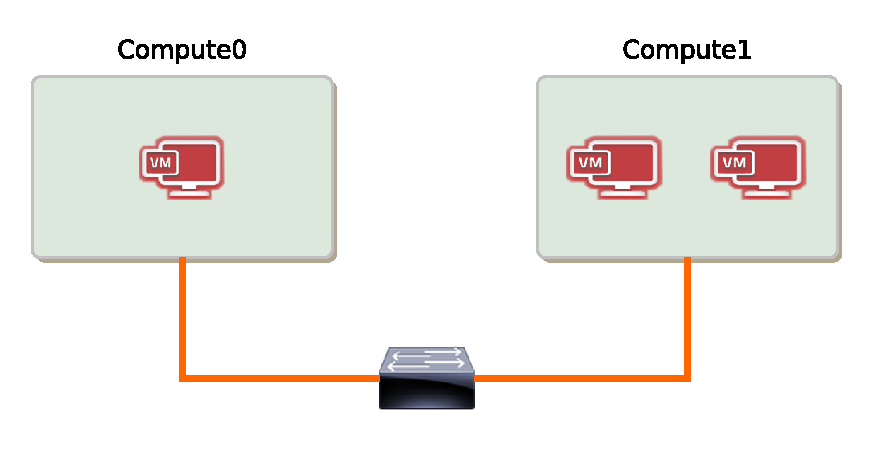
\includegraphics[width=0.8\textwidth]{diagrama.pdf}
    \caption{Esta es una figura que latex decide donde colocar (floating) en el documento.}
    \label{fig:diagrama}
    \end{figure}

  \begin{tabular}{cc}
    Imagen 1 & Imagen 2 \\[2mm]
    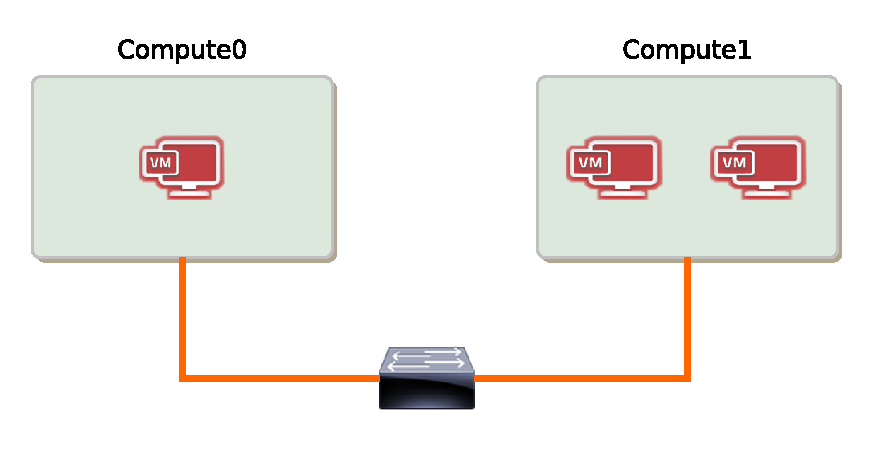
\includegraphics[width=0.4\textwidth]{diagrama.pdf} &  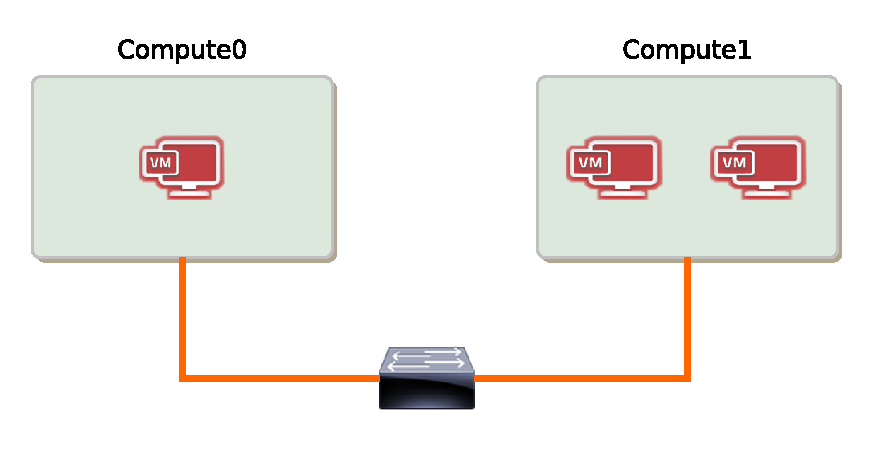
\includegraphics[width=0.4\textwidth]{diagrama.pdf}
  \end{tabular}
  
  Este es un ejemplo de una tabla:
  
  \begin{tabular}{|l|c|}
    \hline
    Columna 1 & Columna 2 \\ \hline
    1 & 2 \\ \hline
  \end{tabular}


  \vspace*{1cm}
  O la misma tabla centrada:

  \begin{center}
    \begin{tabular}{|l|c|}
      \hline
      Columna 1 & Columna 2 \\ \hline
      1 & 2 \\ \hline
    \end{tabular}
  \end{center}

  Para generar el fichero PDF:
  
  \begin{lstlisting}{language=bash}
    pdflatex ejemplo-memoria.tex
    bibtex ejemplo-memoria
    pdflatex ejemplo-memoria.tex
\end{lstlisting}

  También se puede usar \texttt{latexmk} que automáticamente regenera la bibliografía.
  \begin{lstlisting}{language=bash}
    latexmk -pdf ejemplo-memoria.tex
\end{lstlisting}

  

\addcontentsline{toc}{chapter}{Bibliografía}
\bibliographystyle{unsrt}
\bibliography{bib/bibliografia}




\end{document}

%%% Local Variables:
%%% mode: latex
%%% TeX-master: t
%%% End:
